\chapter{Probability Theory}

\section{Random Variables}
Given a random variable $X$, one may generate other random variables by applying various transformations on $X$. As an example, Y is a \textbf{linear} function of $X$, of the form

\begin{equation}
    Y = g(x) = aX + b
\end{equation}

where $a$ and $b$ are given scalars.

If $Y = g(X)$ is a function of a random variable $X$, then $Y$ is also a random variable, since it provides a numerical value for each possible outcomes. This is because every outcome in the sample space defines a numerical value $x$ for $X$ and hence also the numerical value $y = g(x)$ for $Y$.

If $X$ is discrete with PMF $p_X$, then $Y$ is also discrete, and its PMF $p_Y$ can be calculated using the PMF of $p_X$. To obtain $p_Y(y)$ for any $y$, we add the probabilities of all value $x$ such that $g(x) = y$

\begin{equation}
    p_Y(y) = \sum_{x | g(x) = y} p_X(x)
\end{equation}



\section{Conditional Probability}

Imagine we have two boxes, one red and one blue, and in the red box we have 2 apples and 6 oranges, and in the blue box we have 3 apples and 1 orange.

Now suppose we randomly pick one of the boxes and from that box we randomly select an item of fruit.

Let us suppose that in so doing we pick the red box 40\% of the time and we pick the blue box 60\% of the time.

The identity of the box that will be chosen is a random variable, which we shall denote by $B$. This random variable can take one of two possible values, namely $r$ (red box) or $b$ (blue box).

The identity of the fruit is also a random variable and will be denoted by $F$.  It can take either of the values $a$ (apple) or $o$ (orange).

The probability of selecting the red box is $\frac{4}{10}$ and the probability of selecting the blue box is $\frac{6}{10}$. In other words, $p(B = r) = \frac{4}{10}$ and $p(B = b) = \frac{6}{10}$.

By definition, probabilities must lie in the interval $[0, 1]$. If the events are mutually exclusive and if they include all possible outcomes, then we see that the probabilities for those events must sum to one.

\begin{enumerate}
    \item What is the overall probability that the selection procedure will pick an apple?
    \item Given that we have chosen an orange, what is the probability that the box we chose was the blue one?
\end{enumerate}

\begin{figure}
    \centering
    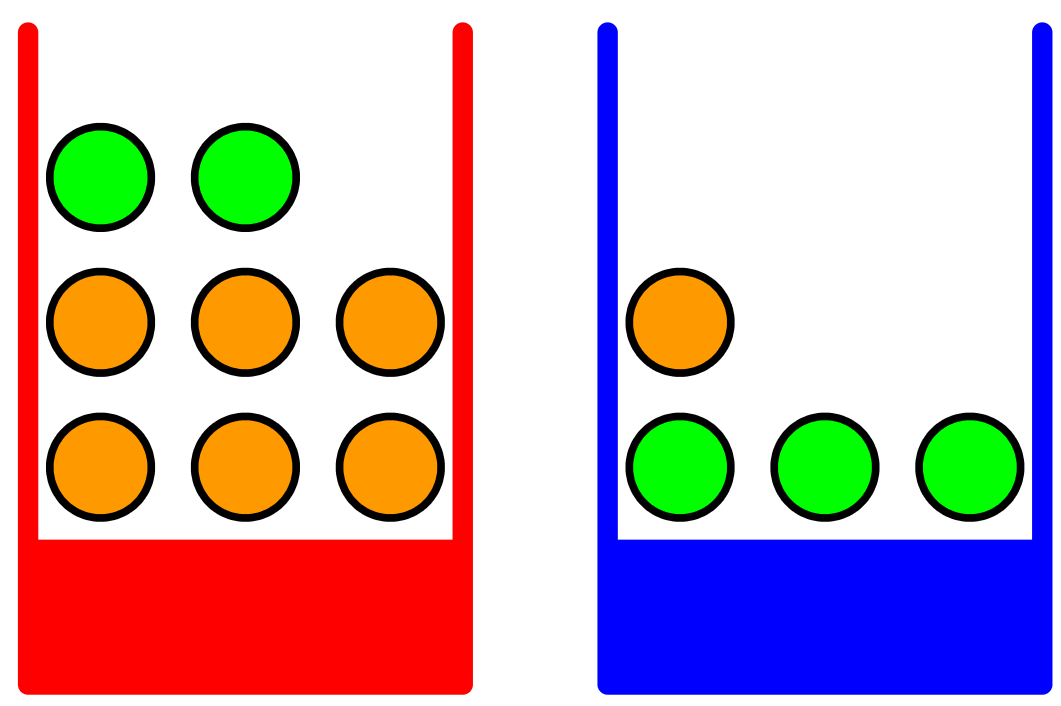
\includegraphics[width=5cm]{chapter008/figures/fig001.png}
    \caption{Line representation}
\end{figure}

We shall suppose that $X$ can take any of the values $x_i$ where $i = 1, ..., M$, and $Y$ can take the values $y_j$ where $j=1, ..., L$.

Consider a total of $N$ trials in which we sample both of the variables $X$ and $Y$, and let the number of such trials in which $X=x_i$ and $Y = y_j$ be $n_{ij}$.

Let the number of trials in which $X$ takes the value $x_i$ be denoted by $c_i$, and similarity let the number of trials in which $Y$ takes the value $y_j$ be denoted by $r_j$

The probability that $X$ will take the value $x_i$ and $Y$ will take the value $y_j$ is written $p(X = x_i, Y = y_j)$ and is called the \textbf{joint probability} of $X = x_i$ and $Y = y_j$, and hence

\begin{equation}
    p(X = x_i, Y = y_j) = \frac{n_{ij}}{N}
\end{equation}

Here we are implicitly considering the limit $N \rightarrow \infty$. Similarity, the probability that $X$ takes the value $x_i$ irrespective of the value of $Y$ is written as $p(X = x_i)$, so that

\begin{equation}
    p(X = x_i) = \frac{c_{ij}}{N}
\end{equation}

\begin{equation}
    p(X = x_i) = \sum_{j=1}^L p(X = x_i, Y = y_j)
\end{equation}

\begin{figure}
    \centering
    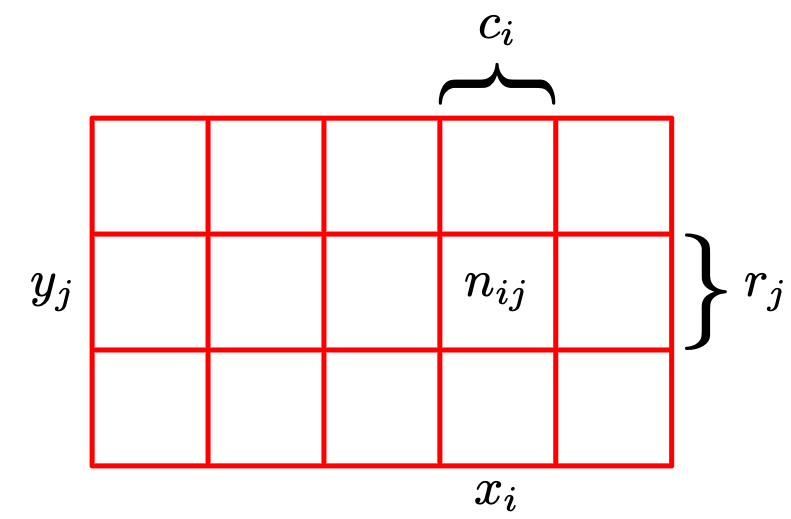
\includegraphics[width=5cm]{chapter008/figures/fig002.png}
    \caption{Join Probability}
\end{figure}

which is the sum rule of probability.  Note that $p(X=x_i)$ is sometimes called the $marginal$ probability, because it is obtained by marginalizing, or summing out.

If we consider only those instances for which $X = x_i$, then the fraction of such instances for which $Y=y_j$ is written $p(Y = y_j | X = x_i)$ and is called the \textbf{conditional} probability of $Y=y_j$ given $X=x_i$. It is obtained by finding the fraction of those points in column $i$ that fall in cell $i,j$ and hence is given by

\begin{equation}
    p(Y = y_j | X = x_i) = \frac{n_{ij}}{c_i}
\end{equation}

then,

\begin{equation}
    \begin{split}
        p(X = x_i, Y = y_j) & = \frac{n_{ij}}{N}\\
        & = \frac{n_{ij}}{c_i} \cdot \frac{c_i}{N}\\
        & = p(Y = y_j | X = x_i)p(X = x_i)
    \end{split}
\end{equation}

which is the \textbf{product rule} of probability.

Here $p(X, Y)$ is a joint probability and is verbalized as "the probability of $X$ and $Y$". The quantity $p(Y | X)$ is a conditional probability and is verbalized as "the probability of $Y$ given $X$", whereas the quantity $p(X)$ is marginal probability and is simply "the probability of $X$"

We have seen that the probabilities of selecting either the red or the blue boxes are given by

\begin{equation}
    p(B = r) = \frac{4}{10}\ \ \ 
    p(B = b) = \frac{6}{10}
\end{equation}

so, $p(B = r) + b(B = b) = 1$. 

Suppose that we pick a box at random, and it turns out to be the blue box. Then the probability of selecting an apple is just the fraction of apples in the blue box which is $3/4$, and so $p(F = a | B = b) = 3/4$. In fact,

$$
    p(F = a | B = r) = \frac{1}{4}\\
    p(F = o | B = r) = \frac{3}{4}\\
    p(F = a | B = b) = \frac{3}{4}\\
    p(F = o | B = b) = \frac{1}{4}\\
$$

and

\begin{equation}
    \begin{split}
        p(F = a) & = p(F = a | B = r)p(B = r) + p(F = a | B = b)p(B = b)\\
        & = \frac{1}{4} \times \frac{4}{10} + \frac{3}{4} \times \frac{6}{10} = \frac{11}{20}
    \end{split}
\end{equation}

if $p(X, Y) = p(X)p(Y)$, then $X$ and $Y$ are said to be independent. If each box contained the same fraction of apples and oranges, then $p(F|B) = P(F)$.


\section{Total Probability Theorem}
Let $A_1, ..., A_n$ be disjoint events that form a partition of the sample space and assume that $P(A_i) > 0$, for all $i$. Then, for any event B, we have

\begin{equation}
    \begin{split}
        P(B) & = P(A_1 \cap B) + ... + P(A_n \cap B)\\
        & = P(A_1)P(B | A_1) + ... + P(A_n)P(B | A_n)
    \end{split}
\end{equation}


\begin{equation}
    B = (A_1 \cap B) \cup ... \cup (A_n \cap B)
\end{equation}

Using the additivity axiom, it follows that

\begin{equation}
    P(B) = P(A_1 \cap B) + ... + P(A_n \cap B)
\end{equation}

by the definition of conditional probability, we have
\begin{equation}
    P(A_i \cap B) = P(A_i)P(B | A_i)
\end{equation}

then,
\begin{equation}
   P(B) = P(A_1)P(B | A_1) + ... + P(A_n)P(B | A_n)
\end{equation}


\section{Bayes' Theorem}

\begin{equation}
    p(Y|X) = \frac{p(X|Y)p(Y)}{p(X)}
\end{equation}

where

\begin{equation}
    p(X) = \sum_{Y} p(X|Y)p(Y)
\end{equation}

Suppose we are told that a piece of fruit has been selected and it is an orange, and we would like to know which box it came from. This requires that we evaluate the probability distribution over boxes conditioned on the identity of the fruit.

We can solve the problem of reversing the conditional probability by using Bayes's theorem to give

\begin{equation}
    p(B = r | F = 0) = \frac{p(F = o | B = r)p(B = r)}{p(F = o)} = \frac{3}{4} \times \frac{4}{10} \times \frac{20}{9} = \frac{2}{3}
\end{equation}

If we had been asked which box had been chosen before being told the identity of the selected item of fruit, then the most complete information we have available is provided by the probability $p(B)$ which is called \textbf{prior probability} because it is the probability available \textbf{before} we observe the identity of the fruit. Once we are told that the fruit is an orange, we can then use Bayes' theorem to compute the probability $p(B | F)$, which is shall call the \textbf{posterior probability}, because it is the probability obtained  \textbf{after} we have observed F.

Let $A_1, A_2, ..., A_n$ be disjoint events that form a partition of the sample space, and assume that $P(A_i) > 0$, for all $i$. Then, for any event B such that $P(B) > 0$, we have

\begin{equation}
    \begin{split}
        P(A_i | B) & = \frac{P(A_i)P(B | A_i)}{P(B)}\\
        & = \frac{P(A_i)P(B | A_i)}{P(A_1)P(B | A_1) + ... + P(A_n)P(B|A_n)}
    \end{split}
\end{equation}

\section{Exercise}

\subsection{Exercise 1}
You enter a chess tournament where your probability of winning a game is $0.3$ against half the players (call them type 1), 0.4 against a quarter of the players (call them type 2), and 0.5 against the remaining quarter of the players (call them type 3). You play a game against a randomly chosen opponent. What is the probability of wining?

Let $A_i$ be the \textbf{event of playing with} an opponent of type $i$. We have
$$
    P(A_1) = 0.5, P(A_2) = 0.25, P(A_3) = 0.25
$$

Also, let B be the event of winning. We have

$$
    P(B | A_1) = 0.3, P(B | A_2) = 0.4, P(B | A_3) = 0.5
$$

Thus, the probability of winning is

\begin{equation}
    \begin{split}
        P(B) & = P(A_1)P(B | A_1) + P(A_2)P(B|A_2) + P(A_3)P(B|A_3)\\
        & = 0.5 \cdot 0.3 + 0.25 \cdot 0.4 + 0.25 \cdot 0.5\\
        & = 0.375
    \end{split}
\end{equation}

\section{Expectations}

One of the most important operations involving probabilities is that of finding weighted averages of functions. The average value of some function $f(x)$ under a probability distribution $p(x)$ is called the \textbf{expectation} of $f(x)$ and will be denoted by $\mathbb{E}[f]$

\begin{equation}
    \mathbb{E}[f] = \sum_x p(x)f(x)
\end{equation}

so that the average is weighted by the relative probabilities of the different values of $x$.

\begin{equation}
    \mathbb{E}[f] = \int p(x)f(x)dx
\end{equation}

In either case, if we are given a finite number $N$ of points drawn from the probability distribution or probability density, then the expectation can be approximated as a finite sum over these points. 

\begin{equation}
       \mathbb{E}[f] \simeq \frac{1}{N}\sum_{n=1}^N f(x_n) 
\end{equation}

The approximation becomes exact in the limit $N \rightarrow \infty$.

\section{Conditional Expectation}

\begin{equation}
    \mathbb{E}[f | y] = \sum_x p(x | y)f(x)
\end{equation}

\section{Properties of Mean and Variance}

Given $a$ and $b$ are scalars,

\begin{equation}
    \begin{split}
        \mathbb{E}[aX + b] & = \sum_x (ax + b)p_X(x)\\
         & = a \sum_x xp_X(x) + b\sum_x p_X(x)\\
         & = a \mathbb{E}[X] + b
    \end{split}
\end{equation}

because $\sum_x p_X(x) = 1$

\section{Variance}

\begin{equation}
    \begin{split}
        var[X] & = \mathbb{E}[(X - \mu])^2]\\
        & = \sum_x (x - \mu)^2p_X(x)\\
        & = \sum_x(x^2 -2x\mu + \mu^2)p_X(x)\\
        & = \sum_xx^2p_X(x) - \sum_x 2x \mu p_X(x) + \sum_x \mu^2p_X(x)\\
        & = \sum_xx^2p_X(x) - 2\mu \sum_x x p_X(x) + \mu^2\sum_x p_X(x)\\
        & = E[X^2] - 2\mu^2 + \mu^2\\
        & = E[X^2] - \mu^2
    \end{split}
\end{equation}

because $\mu = \mathbb{E}[f(x)$ is just a number and $\sum_x p_X(x) = 1$.

The variance of f(x) provides a measure of how much variability there is in $f(x)$ around its mean value $\mathbb{E}$.

\section{Covariance}
\begin{equation}
    \begin{split}
        cov[x, y] & = \mathbb{E}_{x, y}[\{x - \mathbb{E}[x]\}\{y - \mathbb{E}[y]\}]\\
        & = \mathbb{E}_{x, y}[xy - x\mathbb{E}[y] - y\mathbb{E}[x] + \mathbb{E}[x]\mathbb{E}[y]]\\
        & = \mathbb{E}_{x, y}[xy] - \mathbb{E}_{x, y}[x\mathbb{E}[y]] - \mathbb{E}_{x, y}[y\mathbb{E}[x]] +  \mathbb{E}_{x, y}[\mathbb{E}[x]\mathbb{E}[y]]\\
        & = \mathbb{E}_{x, y}[xy] - \mathbb{E}[y]\mathbb{E}_{x, y}[x] - \mathbb{E}[x]\mathbb{E}_{x, y}[y] + \mathbb{E}[x]\mathbb{E}[y]\\
        & = \mathbb{E}_{x, y}[xy] - 2\mathbb{E}[x]\mathbb{E}[y] + \mathbb{E}[x]\mathbb{E}[y]\\
        & = \mathbb{E}_{x, y}[xy] - \mathbb{E}[x]\mathbb{E}[y]
    \end{split}
\end{equation}

if $x$ and $y$ are independent, then their covariance vanishes.

In the case of two vectors of random variables $x$ and $y$, the covariance is a matrix

\begin{equation}
    \begin{split}
        cov[x, y] & = \mathbb{E}_{x, y}[\{x - \mathbb{E}[x]\}\{y^T -  \mathbb{E}[y^T]\}]\\
        & = \mathbb{E}_{x, y}[xy^T] - \mathbb{E}[x]\mathbb{E}[y^T]
    \end{split}
\end{equation}

Note that each data point is a vector, then average of multiple vectors is also a vector.

\section{The Gaussian Distribution}
It is also called \textbf{normal} distribution. For the case of a single real-valued variable $x$, the Gaussian distribution is defined by

\begin{equation}
    \mathcal{N}(x | \mu, \sigma^2) = \frac{1}{(2\pi \sigma ^2)^{1/2}} e^{-\frac{1}{2\sigma^2}(x - \mu)^2}
\end{equation}

which is governed by two parameters: $\mu$, called \textbf{mean}, and $\sigma^2$, called the \textbf{variance}. The square root of the variance, given by $\sigma$, is called the \textbf{standard deviation}, and the reciprocal of the variance, written as $\beta = \frac{1}{\sigma^2}$, is called the precision.

The Gaussian distribution satisfies

\begin{equation}
    \mathcal{N}(x | \mu, \sigma^2) > 0
\end{equation}

Let 

\begin{equation}
    I = \int_{- \infty}^{\infty} exp(- \frac{1}{2 \sigma^2}x^2)dx 
\end{equation}

then,

\begin{equation}
    \begin{split}
        I^2 & = \int_{- \infty}^{\infty} \int_{- \infty}^{\infty} exp(- \frac{1}{2 \sigma^2}x^2) exp(- \frac{1}{2 \sigma^2}y^2)dxdy\\
        & = \int_{- \infty}^{\infty} \int_{- \infty}^{\infty} exp(- \frac{1}{2 \sigma^2}x^2 - \frac{1}{2 \sigma^2}y^2 )dxdy\\
        & = \int_{- \infty}^{\infty} \int_{- \infty}^{\infty} exp(- \frac{1}{2 \sigma^2}(x^2 + y^2) )dxdy\\
    \end{split} 
\end{equation}

Let
$$
    x = rcos \theta, y = r sin \theta
$$
 
then,

\begin{align*}
    \frac{\partial(x, y)}{\partial (r, \theta)} = 
    \begin{vmatrix}
        \frac{\partial x}{\partial r} & \frac{\partial x}{\partial \theta}\\
        \frac{\partial y}{\partial r} & \frac{\partial y}{\partial \theta}
    \end{vmatrix}dr d\theta
    =
    \begin{vmatrix}
        \cos \theta & -r\sin \theta\\
        \sin \theta & r \cos \theta
    \end{vmatrix} dr d \theta = 
    r (\cos \theta)^2 + r (\sin \theta)^2drd \theta = rdrd\theta
\end{align*}

based on the fact:

\begin{equation}
    \begin{split}
        \int_{- \infty}^{\infty} exp(-\frac{r^2}{2\sigma^2})rdr
    \end{split}
\end{equation}

let $u = -\frac{r^2}{2\sigma^2}$, then

\begin{equation}
    du = -\frac{r}{\sigma^2}dr \Leftrightarrow -\sigma^2du = rdr
\end{equation}

then,

\begin{equation}
    \begin{split}
        \int_{- \infty}^{\infty} exp(-\frac{r^2}{2\sigma^2})rdr = -\sigma^2\int_{- \infty}^{\infty} exp(u)du = - \sigma^2 exp(u) |_0^{+\infty} = - \sigma^2 exp(-\frac{r^2}{2\sigma^2}) |_0^{+\infty}
    \end{split}
\end{equation}

because

$$
    exp(-\frac{r^2}{2\sigma^2}) = e^{-\frac{r^2}{2\sigma^2}} = \frac{1}{e^{\frac{r^2}{2\sigma^2}}} = 0 \ when\ r \rightarrow \infty
$$

thus

$$
    - \sigma^2 exp(-\frac{r^2}{2\sigma^2}) |_0^{+\infty} = -\sigma^2(0 - 1) = \sigma^2
$$

Note that in the trigonometry circle, the radius=1 and $cos \theta = r$, then

\begin{equation}
    \begin{split}
        y & = rsin\theta\\
        \Leftrightarrow dy & = sin \theta dr\\
        \Leftrightarrow dxdy & = cos \theta drd\theta\\
        \Leftrightarrow dxdy & = r drd\theta
    \end{split}
\end{equation}

\begin{equation}
    \begin{split}
        I^2 & = \int_{0}^{2 \pi} \int_{- \infty}^{\infty} exp(- \frac{1}{2 \sigma^2}(x^2 + y^2) )dxdy\\
        & = \int_{0}^{2 \pi} \int_{- \infty}^{\infty} exp(- \frac{1}{2 \sigma^2}r^2 )r drd\theta\\
        & = \int_{0}^{2 \pi} \sigma^2 d\theta\\
        & = \theta \sigma^2 |_{0}^{2\pi} = 2 \pi \sigma^2\\
        \Leftrightarrow I & = \sqrt{2 \pi}\sigma
    \end{split}
\end{equation}

Finally, let $y = x - \mu \Leftrightarrow dy = dx$

\begin{equation}
    \begin{split}
        \int_{- \infty}^{\infty} \mathcal{N}(x | \mu, \sigma^2)dx & = \int_{- \infty}^{\infty} \frac{1}{(2\pi \sigma ^2)^{1/2}} e^{-\frac{1}{2\sigma^2}(x - \mu)^2}dx\\
        & = \int_{- \infty}^{\infty} \frac{1}{(2\pi \sigma ^2)^{1/2}} e^{-\frac{1}{2\sigma^2}y^2}dy\\
        & = \frac{1}{(2\pi \sigma ^2)^{1/2}} \int_{- \infty}^{\infty} e^{-\frac{1}{2\sigma^2}y^2}dy\\
        & = \frac{I}{(2\pi \sigma ^2)^{1/2}}\\
        & = 1
    \end{split}
\end{equation}

Because the parameter $\mu$ represents the average value of $x$ under the distribution, it is referred as the mean

\begin{equation}
    \mathbb{E}[x] = \int_{- \infty}^{\infty} \mathcal{N}(x | \mu, \sigma^2)xdx = \mu
\end{equation}

To proof that, we need to know that

\begin{align}
    \begin{split}
        \int_{-a}^{a} f(x)dx & = \int_{-a}^{0} f(x)dx + \int_{0}^{a} f(x)dx\\
        & = - \int_{0}^{-a} f(x)dx + \int_{0}^{a} f(x)dx
    \end{split}
\end{align}

Let $u = -x$, then $du = -dx$ and $x = -a$, then $u = a$. Thus,

\begin{align}
    \begin{split}
        - \int_{0}^{-a} f(x)dx & = - \int_{0}^{a}  f(-u)(-du)\\
        & = \int_{0}^{a} f(-u)du
    \end{split}
\end{align}

In other words,

\begin{align}
    \begin{split}
        \int_{-a}^{a} f(x)dx & = \int_{0}^{a}  f(-u)(du) + \int_{0}^{a} f(x)dx\\
    \end{split}
\end{align}

If $f$ is odd, then $f(-u) = -f(u)$

\begin{align}
    \begin{split}
        \int_{-a}^{a} f(x)dx & = -\int_{0}^{a}  f(u)(du) + \int_{0}^{a} f(x)dx\\
        & = 0
    \end{split}
\end{align}

So we have,

\begin{align}
    \begin{split}
        \mathbb{E}[x] & = \int_{- \infty}^{\infty} \mathcal{N}(x | \mu, \sigma^2)xdx\\
        & = \int_{- \infty}^{\infty} \frac{1}{(2\pi \sigma ^2)^{1/2}} e^{-\frac{1}{2\sigma^2}(x - \mu)^2}xdx
    \end{split}
\end{align}

Let $y = x - \mu$,  then $x = y + \mu$ and $dy = dx$. We have

\begin{align}
    \begin{split}
        \mathbb{E}[x] & = \int_{- \infty}^{\infty} \mathcal{N}(x | \mu, \sigma^2)xdx\\
        & = \int_{- \infty}^{\infty} \frac{1}{(2\pi \sigma ^2)^{1/2}} e^{-\frac{1}{2\sigma^2}(y)^2}(y + \mu)dy\\
        & = \int_{- \infty}^{\infty} \frac{1}{(2\pi \sigma ^2)^{1/2}} e^{-\frac{1}{2\sigma^2}(y)^2}ydy + \int_{- \infty}^{\infty} \frac{1}{(2\pi \sigma ^2)^{1/2}} e^{-\frac{1}{2\sigma^2}(y)^2}\mu dy\\
    \end{split}
\end{align}

Because

\begin{align}
    \begin{split}
        \frac{1}{(2\pi \sigma ^2)^{1/2}} e^{-\frac{1}{2\sigma^2}(-y)^2}(-y) = - \frac{1}{(2\pi \sigma ^2)^{1/2}} e^{-\frac{1}{2\sigma^2}(y)^2}(y)
    \end{split}
\end{align}

so $\frac{1}{(2\pi \sigma ^2)^{1/2}} e^{-\frac{1}{2\sigma^2}(y)^2}y$ is an odd function. Thus,


$$
    \int_{- \infty}^{\infty} \frac{1}{(2\pi \sigma ^2)^{1/2}} e^{-\frac{1}{2\sigma^2}(y)^2}ydy = 0
$$

We have

$$
    \int_{- \infty}^{\infty} \frac{1}{(2\pi \sigma ^2)^{1/2}} e^{-\frac{1}{2\sigma^2}(y)^2}dy = 1
$$
so,

\begin{equation}
    \mathbb{E}[x] = \int_{- \infty}^{\infty} \mathcal{N}(x | \mu, \sigma^2)xdx = \mu
\end{equation}

Next,

\begin{align}
    \begin{split}
        \mathbb{E}[(x - \mu)^2] & = \int_{- \infty}^{\infty} (x - \mu)^2 \mathcal{N}(x | \mu, \sigma^2)dx\\
        & = \frac{1}{\sigma\sqrt{2\pi}}\int_{- \infty}^{\infty} (x - \mu)^2 exp(- \frac{1}{2 \sigma^2}(x - \mu)^2)dx
    \end{split}
\end{align}

Let
\begin{align}
        y = x - \mu \Leftrightarrow dy = dx  \qquad    x = y + \mu
\end{align}

so,

\begin{align}
    \begin{split}
        \mathbb{E}[(x - \mu)^2] & = \int_{- \infty}^{\infty} (x - \mu)^2 \mathcal{N}(x | \mu, \sigma^2)dx\\
        & = \frac{1}{\sigma\sqrt{2\pi}}\int_{- \infty}^{\infty} y^2 exp(- \frac{1}{2 \sigma^2}y^2)dx
    \end{split}
\end{align}

let

\begin{equation}
    \begin{cases}
      u & = y\\
      v & = - \sigma ^ 2 e^{- \frac{y^2}{2 \sigma^2}}\\
    \end{cases}
    \Leftrightarrow
    \begin{cases}
      du & = dy\\
      dv & = - \sigma ^ 2 (-\frac{2y}{2 \sigma ^2}) e^{- \frac{y^2}{2 \sigma^2}}dy\\
    \end{cases}
    \Leftrightarrow
    \begin{cases}
      du & = dy\\
      dv & = y e^{- \frac{y^2}{2 \sigma^2}}dy\\
    \end{cases}
\end{equation}

Applying Formula for Integration by Parts, we have
\begin{equation}
    \begin{split}
        \int u dv & = u v - \int v du\\
        & = y (- \sigma ^ 2 e^{- \frac{y^2}{2 \sigma^2}})|_{- \infty}^{\infty} - \int - \sigma ^ 2 e^{- \frac{y^2}{2 \sigma^2}}du\\
        & = y (- \sigma ^ 2 e^{- \frac{y^2}{2 \sigma^2}})|_{- \infty}^{\infty} + \int \sigma ^ 2 e^{- \frac{y^2}{2 \sigma^2}}dy
    \end{split}
\end{equation}

then,

\begin{align}
    \begin{split}
        \mathbb{E}[(x - \mu)^2] & = \frac{1}{\sigma\sqrt{2\pi}}y (- \sigma ^ 2 e^{- \frac{y^2}{2 \sigma^2}})|_{- \infty}^{\infty} + \frac{1}{\sigma\sqrt{2\pi}}\int \sigma ^ 2 e^{- \frac{y^2}{2 \sigma^2}}dy\\
        & = \frac{1}{\sigma\sqrt{2\pi}}y (- \sigma ^ 2 e^{- \frac{y^2}{2 \sigma^2}})|_{- \infty}^{\infty} + \sigma ^ 2\int \frac{1}{\sigma\sqrt{2\pi}} e^{- \frac{y^2}{2 \sigma^2}}dy\\
        & = 0 + \sigma ^ 2 \cdot 1\\
        & = \sigma^2
    \end{split}
\end{align}

Note that 
$$
    \frac{1}{\sigma\sqrt{2\pi}}y (- \sigma ^ 2 e^{- \frac{y^2}{2 \sigma^2}})
$$

approach to $0$ when $y$ approach to $\infty$.

Given a $D$-dimensional vector $x$ of continuous variables, we have

\begin{equation}
    \mathcal{N}(x | \mu, \Sigma) = \frac{1}{(2\pi)^{D/2}} \frac{1}{|\Sigma|^{1/2}}exp\{-\frac{1}{2}(x - \mu)^T\Sigma^-1(x - \mu)\}
\end{equation}

where the $D$-dimensional vector $\mu$ is called the mean, the $D \times D$ matrix $\Sigma$ is called the covariance, and $|\Sigma|$ denotes the determinant of $\Sigma$.

\section{Maximum Likelihood}

Now suppose that we have a data set of observations $X = (x_1, ..., X_N)^T$, representing $N$ observations of the scalar variable $x$. We suppose that the observations are drawn independent from a Gaussian distribution whose $\mu$ and $\sigma^2$ are unknown, and we would like to determine these parameters from the dataset.

Data points that are drawn independently from the same distribution are said to be \textbf{independent and identically distributed (iid)}.

Because our data set $X$ is $i.i.d$, we can therefore write the probability of the data set, given $\mu$ and $\sigma^2$, in the form

\begin{equation}
    p(X|\mu, \sigma^2) = \prod_{n=1}^N \mathcal{N}(x_n|\mu, \sigma^2)
\end{equation}

One common criterion for determining the parameters in a probability distribution using an observed data set is to find the parameter values that maximize the likelihood function. This might seem like a strange criterion because, it would seem more natural to maximize the probability of the parameters given the data, not the probability of the data given the parameters.

In practice, it is more convenient to maximize the log of the likelihood function. because the logarithm is a \textbf{monotonically increasing} function of its argument, maximization of the log of a function is equivalent to maximization of the function itself.

\begin{align}
    \begin{split}
        p(X|\mu, \sigma^2) & = \prod_{n=1}^N \mathcal{N}(x_n|\mu, \sigma^2)\\
        \Leftrightarrow ln\{p(X|\mu, \sigma^2)\} & = \sum ln \{\mathcal{N}(x_n|\mu, \sigma^2)\}\\
        & = \sum_{n=1}^N ln(\frac{1}{(2\pi \sigma^2)^{1/2}}exp\{-\frac{1}{2\sigma ^ 2}(x_n - \mu)^2\})\\
        & = \sum_{n=1}^N ln(\frac{1}{(2\pi \sigma^2)^{1/2}} + \sum_{n=1}^N ln(exp\{-\frac{1}{2\sigma ^ 2}(x_n - \mu)^2\}))\\
        & = \sum_{n=1}^N ln(1) - \sum_{n=1}^N ln((2\pi \sigma^2)^{1/2}) + \sum_{n=1}^N -\frac{1}{2\sigma ^ 2}(x_n - \mu)^2\ ln(e)\\
        & = - \frac{1}{2} \sum_{n=1}^N ln((2\pi \sigma^2) - \sum_{n=1}^N \frac{1}{2\sigma ^ 2}(x_n - \mu)^2\\
        & = - \frac{1}{2} \sum_{n=1}^N ln(2 \pi) - \frac{1}{2} \sum_{n=1}^N ln(\sigma^2) - \sum_{n=1}^N \frac{1}{2\sigma ^ 2}(x_n - \mu)^2\\
        & = - \frac{1}{2\sigma ^ 2}\sum_{n=1}^N (x_n - \mu)^2 - \frac{N}{2} ln(2 \pi) - - \frac{N}{2} ln(\sigma^2)
    \end{split}
\end{align}

The $lnp(X|\mu, \sigma^2)$ is maximized $\Leftrightarrow \frac{\partial ln\{p(X|\mu, \sigma^2)\}}{\partial \mu} = 0$, then we have

\begin{align}
    \begin{split}
        \frac{\partial ln\{p(X|\mu, \sigma^2)\}}{\partial \mu} & = 0\\
        \Leftrightarrow - \frac{1}{2\sigma ^ 2} \sum_{n=1}^N (-2x_n + 2\mu) & = 0\\
        \Leftrightarrow \sum_{n=1}^N (-2x_n + 2\mu) & = 0\\
        \Leftrightarrow \sum_{n=1}^N \mu & = \sum_{n=1}^N x_n\\
        \Leftrightarrow N \mu & = \sum_{n=1}^N x_n\\
        \Leftrightarrow \mu_{ML} & = \frac{1}{N}\sum_{n=1}^N x_n
    \end{split}
\end{align}

$\mu_{ML}$ is the \textbf{sample mean}, the mean of the observed values $\{x_n\}$.

Maximizing $lnp(X|\mu, \sigma^2)$ with respect to $\sigma$, we have

\begin{align}
    \begin{split}
        \frac{\partial ln\{p(X|\mu, \sigma^2)\}}{\partial \mu} & = 0\\
        \Leftrightarrow - \frac{-2}{2 \sigma^3} \sum_{n=1}^N (x_n - \mu)^2 - \frac{N}{2} \frac{2\sigma}{\sigma^2} & = 0\\
        \Leftrightarrow \frac{1}{\sigma^3} \sum_{n=1}^N (x_n - \mu)^2 & = \frac{N}{\sigma}\\
        \Leftrightarrow \sum_{n=1}^N (x_n - \mu)^2 & = N \sigma ^ 2\\
        \Leftrightarrow \sigma^2 & = \frac{1}{N} \sum_{n=1}^N (x_n - \mu)^2\\
        \Rightarrow \sigma^2 & = \frac{1}{N} \sum_{n=1}^N (x_n - \mu_{ML})^2 
    \end{split}
\end{align}

which is the sample variance measured with respect to the sample mean $\mu_{ML}$.

\begin{align}
    \begin{split}
        \mathbb{E}[\mu_{ML}] & = \mathbb{E}[\frac{1}{N}\sum_{n=1}^N x_n]\\
        & = \frac{1}{N}\mathbb{E}[\sum_{n=1}^N x_n]\\
        & = \frac{1}{N}\mathbb{E}[x_1 + x_2 + ... + x_N]\\
        & = \frac{1}{N}(\mathbb{E}[x_1] + \mathbb{E}[x_2] + ... + \mathbb{E}[x_N])\\
        & = \frac{N}{N}(\mathbb{E}[x_n])\\
        & = \mathbb{E}[x_n]\\
        & = \mu
    \end{split}
\end{align}


\begin{align}
    \begin{split}
        \mathbb{E}[\sigma^2_{ML}] & = \mathbb{E}[\frac{1}{N}\sum_{n=1}^N (x_n - \mu_{ML})^2]\\
        & = \frac{1}{N}\mathbb{E}[\sum_{n=1}^N (x_n - \mu_{ML})^2]\\
        & = \frac{1}{N}\mathbb{E}[\sum_{n=1}^N x_n^2 - 2x_n\mu_{ML} + \mu_{ML}^2]\\
        & = \frac{1}{N}\mathbb{E}[\sum_{n=1}^N x_n^2] - \frac{1}{N}\mathbb{E}[\sum_{n=1}^N 2x_n\mu_{ML}] + \frac{1}{N}\mathbb{E}[\sum_{n=1}^N\mu_{ML}^2]\\
        & = \frac{1}{N}\mathbb{E}[\sum_{n=1}^N x_n^2] - \frac{2}{N}\mathbb{E}[\sum_{n=1}^N x_n\mu_{ML}] + \frac{1}{N}\mathbb{E}[N\mu_{ML}^2]\\
        & = \frac{1}{N}\mathbb{E}[\sum_{n=1}^N x_n^2] - \frac{2}{N}\mathbb{E}[\sum_{n=1}^Nx_n\mu_{ML}] + \mathbb{E}[(\frac{1}{N} \sum_{n=1}^N x_n)^2]\\
        & = \frac{1}{N}\mathbb{E}[\sum_{n=1}^N x_n^2] - \frac{2}{N}\mathbb{E}[\sum_{n=1}^Nx_n\mu_{ML}] + (\frac{1}{N})^2 \mathbb{E}[(\sum_{n=1}^N x_n)^2\\
        & = \frac{1}{N}\mathbb{E}[\sum_{n=1}^N x_n^2] - \frac{2}{N}\mathbb{E}[\sum_{n=1}^Nx_n \frac{1}{N}\sum_{n=1}^Nx_n] + (\frac{1}{N})^2 \mathbb{E}[(\sum_{n=1}^N x_n)^2\\
        & = \frac{1}{N}\mathbb{E}[\sum_{n=1}^N x_n^2] - \frac{2}{N^2}\mathbb{E}[\sum_{n=1}^Nx_n \sum_{n=1}^Nx_n] + (\frac{1}{N})^2 \mathbb{E}[(\sum_{n=1}^N x_n)^2\\
        & = \frac{1}{N}\mathbb{E}[\sum_{n=1}^N x_n^2] - \frac{2}{N^2}\mathbb{E}[(\sum_{n=1}^Nx_n)^2] + (\frac{1}{N})^2 \mathbb{E}[(\sum_{n=1}^N x_n)^2]\\
        & = \frac{1}{N}\mathbb{E}[\sum_{n=1}^N x_n^2] - \frac{1}{N^2}\mathbb{E}[(\sum_{n=1}^Nx_n)^2]\\
        & = \frac{1}{N}(N(\mu^2 + \sigma^2)) - \frac{1}{N^2}\mathbb{E}[(\sum_{n=1}^Nx_n)^2]\\
        & = (\mu^2 + \sigma^2) - \frac{1}{N^2}\mathbb{E}[(\sum_{n=1}^Nx_n)^2]\\
    \end{split}
\end{align}

Note that, given $N = 3$

\begin{align}
    \begin{split}
        \sum_{n=1}^3\sum_{m=1}^3 a_na_m & = (a_1 + a_2 + a_3)(a_1 + a_2 + a_3)\\
        & = a_1^2 + a_2^2 + a_3^2 + 2a_1a_3 + 2a_2a_3 + 2a_1a_2\\
    \end{split}
\end{align}

therefore,

\begin{align}
    \begin{split}
        \mathbb{E}[\sum_{n=1}^3\sum_{m=1}^3 a_na_m] & = (\mathbb{E}[a_1^2] + \mathbb{E}[a_2^2] + \mathbb{E}[a_3^2]) + (2\mathbb{E}[a_1a_3] + 2\mathbb{E}[a_2a_3] + 2\mathbb{E}[a_1a_2])\\
        & = 3\mu^2 + 3\sigma^2 + 2\mu^2 + 2\mu^2 + 2\mu^2\\
        & = 9\mu^2 + 3\sigma^2
    \end{split}
\end{align}

thus,
\begin{align}
    \begin{split}
        \mathbb{E}[\sum_{n=1}^N\sum_{m=1}^N a_na_m] & = N^2\mu^2 + N\sigma^2
    \end{split}
\end{align}

so we have

\begin{align}
    \begin{split}
        \mathbb{E}[\sigma^2_{ML}] & = (\mu^2 + \sigma^2) - \frac{1}{N^2}\mathbb{E}[(\sum_{n=1}^Nx_n)^2]\\
        & = (\mu^2 + \sigma^2) - \frac{1}{N^2}(N^2 \mu^2 + N \sigma^2)\\
        & = \sigma^2 - \frac{\sigma^2}{N}\\
        & = \frac{N - 1}{N}\sigma^2
    \end{split}
\end{align}